\documentclass[a4paper]{report}
\usepackage{vntex}
%\usepackage[english,vietnam]{babel}
%\usepackage[utf8]{inputenc}
\usepackage{mathptmx}[ptm]
%\usepackage[utf8]{inputenc}
%\usepackage[francais]{babel}
\usepackage{a4wide,amssymb,epsfig,latexsym,array,hhline,fancyhdr}
\usepackage[normalem]{ulem}
%\usepackage{soul}

\usepackage[makeroom]{cancel}
\usepackage{amsmath}
\usepackage{amsthm}
\usepackage{multicol,longtable,amscd}
\usepackage{diagbox}%Make diagonal lines in tables
\usepackage{booktabs}
\usepackage{alltt}
\usepackage[framemethod=tikz]{mdframed}% For highlighting paragraph backgrounds
\usepackage{caption,subcaption}

\usepackage{lastpage}
\usepackage[lined,boxed,commentsnumbered]{algorithm2e}
\usepackage{enumerate}
\usepackage{color}
\usepackage{float}
\usepackage{graphicx}							% Standard graphics package
\usepackage{array}
\usepackage{tabularx, caption}
\usepackage{multirow}
\usepackage{multicol}
\usepackage{rotating}
\usepackage{graphics}
\usepackage{geometry}
\usepackage{setspace}
\usepackage{epsfig}
\usepackage{tikz}

\usepackage{indentfirst} % Always indent paragraph

\usetikzlibrary{arrows,snakes,backgrounds,calc}
\usepackage[unicode]{hyperref}
\hypersetup{urlcolor=blue,linkcolor=black,citecolor=black,colorlinks=true} 
\usepackage{listings}
%\usepackage{pstcol} 	

\usepackage[table]{xcolor}							% PSTricks with the standard color package

\usepackage[normalem]{ulem}

\newtheorem{theorem}{{\bf Định lý}}
\newtheorem{property}{{\bf Tính chất}}
\newtheorem{proposition}{{\bf Mệnh đề}}
\newtheorem{corollary}[proposition]{{\bf Hệ quả}}
\newtheorem{lemma}[proposition]{{\bf Bổ đề}}
\theoremstyle{definition}
\newtheorem{exer}{Bài toán}
\addtocontents{toc}{\protect\thispagestyle{empty}}
% Remove page number in contents page. 
\addtocontents{lof}{\protect\thispagestyle{empty}}
% Remove page number in list of figure page. 
\addtocontents{lot}{\protect\thispagestyle{empty}}
% Remove page number in list of table page. 
\def\thesislayout{	% A4: 210 × 297
	\geometry{
		a4paper,
		total={160mm,240mm},  % fix over page
		left=30mm,
		top=22mm,
		right=20mm,
		bottom=20mm,
	}
}
\def\thesisheadlayout{	% A4: 210 × 297
	\geometry{
		a4paper,
		total={160mm,240mm},  % fix over page
		left=30mm,
		top=10mm,
	}
}
\thesislayout
\lstset{
	language=R,
	basicstyle=\footnotesize\sffamily,
	commentstyle=\ttfamily\color{black},
	numbers=left,
	numberstyle=\ttfamily\color{black}\footnotesize,
	stepnumber=1,
	numbersep=5pt,
	backgroundcolor=\color{white},
	showspaces=false,
	showstringspaces=false,
	showtabs=false,
	frame=single,
	tabsize=2,
	captionpos=b,
	breaklines=true,
	breakatwhitespace=false,
	title=\lstname,
	escapeinside={},
	keywordstyle={},
	morekeywords={}
}
%\usepackage{fancyhdr}
\setlength{\headheight}{40pt}
\pagestyle{fancy}
\fancyhead{} % clear all header fields
\renewcommand{\footruleskip}{1mm}

\fancyhead[L]{
	\begin{tabular}{rl}
		\begin{picture}(25,15)(0,0)
			\put(0,-8){
\includegraphics[width=10mm, height=10mm]{Images/hcmut.png}}
			%\put(0,-8){
\epsfig{width=10mm,figure=hcmut.eps}}
		\end{picture}&
		%
\includegraphics[width=8mm, height=8mm]{hcmut.png} & %
		\begin{tabular}{l}
			\textbf{  Trường Đại Học Bách Khoa - Đại học Quốc gia TP.HCM }\\
			\textbf{  Khoa Khoa Học \& Kỹ Thuật Máy Tính}
		\end{tabular} 	
	\end{tabular}
}
\fancyhead[R]{
	\begin{tabular}{l}
		\tiny \bf \\
		\tiny \bf 
\end{tabular}  }
\fancyfoot{} % clear all footer fields
\fancyfoot[L]{\scriptsize Báo cáo Đồ án chuyên ngành - HK2 2025 - 2026}
\fancyfoot[R]{\scriptsize Trang {\thepage}/\pageref{LastPage}}


\renewcommand{\headrulewidth}{0.3pt}
\renewcommand{\footrulewidth}{0.3pt}

%Use case specification table
\usepackage{longtable}
\usepackage{array}
\usepackage{caption}
\usepackage{adjustbox} % Or just use the standard geometry/layout packages
\newcommand\tabularhead[1]{
	\setlength{\tabcolsep}{8pt}        % horizontal padding inside cells (default 6pt)
	\renewcommand{\arraystretch}{1.5}  % vertical padding (1.0 default)
	\begin{longtable}{|p{0.12\linewidth}|p{0.7\linewidth}|}
		\caption{Usecase <<#1>>} \\
		\hline
		\textbf{Usecase} & \textbf{#1} \\
		\hline
		\endfirsthead
		\hline
		\textbf{Usecase} & \textbf{#1} \\
		\hline
		\endhead
		\hline
		\endfoot
	}
	
	\newcommand\addrow[2]{#1 &#2\\ \hline}
	
	\newcommand\addmulrow[2]{%
	#1 & \begin{minipage}[t]{\linewidth}%
	\begin{enumerate}%
	#2%
	\end{enumerate}%
	\end{minipage}\\ \hline
	}

	\newcommand\addcondition[2]{%
	#1 & \begin{minipage}[t]{\linewidth}%
	\begin{itemize}%
	#2%
	\end{itemize}%
	\end{minipage}\\ \hline
	}

	\newcommand\addexception[2]{%
	#1 & \begin{minipage}[t]{\linewidth}%
	\begin{enumerate}%
	#2%
	\end{enumerate}%
	\end{minipage}\\ \hline
	}
	
	\newenvironment{usecase}[1]{
		\tabularhead{#1}
	}{
		\end{longtable}
	}


%%%%%%Req counter
% ==== Counter chung cho toàn bộ yêu cầu ====
\newcounter{req}

\makeatletter

% ==== Use Case (US) ====
% #1 = ID thật (A-US03)
% #2 = tên use case
\newcommand{\us}[2]{%
	\refstepcounter{req}% tăng counter req
	\def\@currentlabel{\textbf{#1}}% ép \ref hiển thị ID thật
	\label{us:#1}% ghi label us:A-US03
	\textbf{#1}%
}

% ==== Non-functional Requirement (NFR) ====
% #1 = mã (01)
% #2 = tên
\newcommand{\nfr}[2]{%
	\refstepcounter{req}%
	\def\@currentlabel{\textbf{NFR#1}}% ép \ref hiển thị NFR01
	\label{nfr:#1}%
	\textbf{NRF#1}%
}

\makeatother
	

\setcounter{secnumdepth}{4}
\setcounter{tocdepth}{3}
\makeatletter
\newcounter {subsubsubsection}[subsubsection]
\renewcommand\thesubsubsubsection{\thesubsubsection .\@alph\c@subsubsubsection}
\newcommand\subsubsubsection{\@startsection{subsubsubsection}{4}{\z@}%
	{-3.25ex\@plus -1ex \@minus -.2ex}%
	{1.5ex \@plus .2ex}%
	{\normalfont\normalsize\bfseries}}
\newcommand*\l@subsubsubsection{\@dottedtocline{3}{10.0em}{4.1em}}
\newcommand*{\subsubsubsectionmark}[1]{}
\makeatother

\everymath{\color{black}}%make in-line maths symbols blue to read/check easily

\sloppy
\captionsetup[figure]{labelfont={small,bf},textfont={small,it},belowskip=-1pt,aboveskip=5pt}
%space remove between caption, figure, and text
\captionsetup[table]{labelfont={small,bf},textfont={small,it},belowskip=-1pt,aboveskip=7pt}
\setlength{\floatsep}{5pt plus 2pt minus 2pt}
\setlength{\textfloatsep}{5pt plus 2pt minus 2pt}
\setlength{\intextsep}{10pt plus 2pt minus 2pt}

\thesislayout
	
\begin{document}

\begin{titlepage}
	\begin{tikzpicture}[remember picture, overlay]
		\draw[line width = 4pt] ($(current page.north west) + (0.4in,-0.5in)$) rectangle ($(current page.south east) + (-0.4in,0.5in)$);
		\draw[line width=1.5pt]
		($ (current page.north west) + (0.45in,-0.55in) $)
		rectangle
		($ (current page.south east) + (-0.45in,0.55in) $);
	\end{tikzpicture}
	
	\begin{center}
		\LARGE \textbf{ĐẠI HỌC QUỐC GIA THÀNH PHỐ HỒ CHÍ MINH} \\
		\vspace{0.2cm}
		\LARGE \textbf{TRƯỜNG ĐẠI HỌC BÁCH KHOA} \\
		\vspace{0.2cm}
		\LARGE \textbf{KHOA KHOA HỌC VÀ KĨ THUẬT MÁY TÍNH}
	\end{center}
	
	\vspace{0.3cm}
	
	\begin{figure}[h!]
		\begin{center}
			
\includegraphics[width=4cm]{Images/hcmut.png}
		\end{center}
	\end{figure}
	
	\begin{center}
		\begin{tabular}{c}
			\multicolumn{1}{c}{\textbf{{\LARGE BÁO CÁO}}}\\
			\\{\textbf{{\LARGE ĐỒ ÁN CHUYÊN NGÀNH}}}
			\\
			\\
			\textbf{\LARGE STEAM ANOMALY DETECTION}\\
			\textbf{\LARGE PHÁT HIỆN BẤT THƯỜNG TRÊN STEAM}\\

	
			
		\end{tabular}
	\end{center}
	\vspace{0.5cm}
	\begin{table}[h]
\centering
\begin{tabular}{lll} 
\multicolumn{3}{l}{\textbf{\Large Giáo viên hướng dẫn:} {\Large Huỳnh Văn Thống}}\\
\\
\multicolumn{3}{l}{\textbf{\Large Lớp:} {\Large L01}}\\
\\
\multicolumn{3}{l}{\textbf{\Large Sinh viên thực hiện:}} 
\\
\\
& {\Large Thịnh Trần Khánh Linh} & {\Large 2211862}
\\
\\
& {\Large Trần Quang Tác} & {\Large 2212962}
\end{tabular}
\end{table}
	\vspace{0.5cm}
	\begin{center}
		{\Large TP. HỒ CHÍ MINH, THÁNG 04 NĂM 2026 }
	\end{center}

\end{titlepage}
%\thispagestyle{empty}

\section*{Danh sách thành viên \& đóng góp}

\begin{center}
	\begin{tabularx}{\textwidth}{c l c X c}
		\toprule
		\textbf{STT} & \textbf{Họ và Tên} & \textbf{MSSV} & \textbf{Công việc được giao} & \textbf{Mức độ hoàn thành} \\
		\midrule
		1 & Thịnh Trần Khánh Linh & 2211862 &
		Xây dựng Machine Learning Model, Đánh giá &
		100\% \\
		
		2 & Trần Quang Tác & 2212962 &
		EDA, Visualization, Kiểm thử hệ thống &
		100\% \\
		\bottomrule
	\end{tabularx}

\end{center}


\newpage
\tableofcontents
\newpage
\listoffigures
\newpage
\listoftables
\newpage
\setcounter{page}{1}

%%%%%%%%%%%%%%%%%CONTENTS%%%%%%%%%%%%%%%%%%%
\chapter{Nguồn gốc dữ liệu}

% TODO: Nguồn gốc dữ liệu
\newpage
\chapter{Datawarehouse}

Hệ thống Datawarehouse được xây dựng trên PostgreSQL, lấy điểm nhấn từ mô hình sao (Star Schema). 
Dựa vào các kịch bản \texttt{SQL\_Postgres\_InitWarehouse.sql} và \texttt{SQL\_SQLServer\_CreateStagingDB.sql}, hệ thống bao gồm:
\begin{itemize}
    \item \textbf{Staging Area}: SQL Server. Lưu trữ các bảng \texttt{stg\_players}, \texttt{stg\_history}, \texttt{stg\_reviews}, \texttt{stg\_library\_raw}.
    \item \textbf{Data Warehouse}: PostgreSQL. Có các Dimension (\texttt{dim\_player}, \texttt{dim\_game}, \texttt{dim\_date}) và Fact (\texttt{fact\_game\_play}, \texttt{fact\_player\_review}).
    \item \textbf{Datamart}: Bản \texttt{dm\_steam\_player\_features\_v1} lưu trữ toàn bộ feature phục vụ học máy.
\end{itemize}

\newpage
\section{Tiền xử lý và Tích hợp dữ liệu (ETL Pipeline)}

\subsection{Kiến trúc Tổng quan Hệ thống ETL}

Quá trình tiền xử lý, chuẩn hóa và tích hợp dữ liệu từ các nguồn phân tán được tự động hóa hoàn toàn thông qua nền tảng \textbf{Pentaho Data Integration (PDI / Spoon)}. Kiến trúc luồng dữ liệu được thiết kế chặt chẽ theo mô hình 3 lớp tiêu chuẩn nhằm tối ưu hóa hiệu năng, bảo đảm tính toàn vẹn và khả năng mở rộng của hệ thống:
\begin{enumerate}
    \item \textbf{Vùng tiếp nhận (Landing Zone - định dạng CSV):} Điểm tập kết ban đầu của các tệp dữ liệu thô nguyên bản (RAW CSV) trích xuất từ các bộ dữ liệu gốc, đồng thời liên tục tiếp nhận các gói dữ liệu mới khai thác (crawled data) từ luồng luân chuyển của Steam Crawler. Dữ liệu thô luân chuyển được tổ chức phân vùng thư mục hạ tầng theo cú pháp \texttt{Datasets/landing/extract\_dt=YYYYMMDD/} chứa các tệp trọng tâm như \texttt{players.csv}, \texttt{history.csv}, \texttt{reviews.csv}, \texttt{purchased\_games.csv}, \texttt{private\_steamids.csv}, \texttt{achievements.csv}, và \texttt{games.csv}.
    \item \textbf{Vùng đệm tiền xử lý (Staging Area - MSSQL):} Đóng vai trò là phân vùng đệm trung gian chứa dữ liệu tạm thời, cô lập luồng dữ liệu thô trước khi can thiệp sâu. Vùng Staging được thiết lập cơ chế tự động làm sạch triệt để sau mỗi chu kỳ nạp dữ liệu thành công, bảo đảm tối ưu hóa tài nguyên lưu trữ và tránh xung đột dữ liệu giữa các phiên làm việc.
    \item \textbf{Kho dữ liệu trung tâm (Data Warehouse - PostgreSQL):} Nơi lưu trữ dữ liệu tập trung đã qua xử lý, làm sạch và chuẩn hóa cấu trúc.
\end{enumerate}

\begin{figure}[H]
    \centering
    \IfFileExists{Images/Pentaho/full_run.png}{
        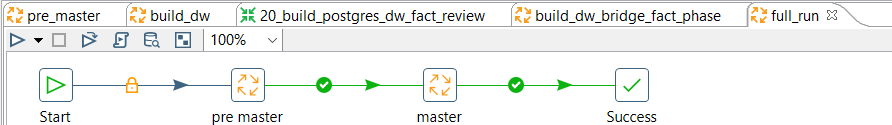
\includegraphics[width=0.9\linewidth]{Images/Pentaho/full_run}
    }{
        \fbox{\begin{minipage}{0.9\linewidth}
            \centering
            \vspace{2cm}
            [IMAGE PLACEHOLDER]\\
            \texttt{Images/Pentaho/full\_run.png}\\
            \vspace{2cm}
        \end{minipage}}
    }
    \caption{Toàn cảnh quá trình thực thi Full Run Pipeline}
    \label{fig:pentaho_full_run}
\end{figure}

Quá trình chạy toàn bộ hệ thống (Full Run) bao gồm hai luồng chính chạy nối tiếp nhau: luồng nạp gốc \textbf{Pre-Master} và luồng tự động hóa \textbf{Master}.

\subsection{Chi tiết Kiến trúc các Luồng Thực thi}

\subsubsection{Luồng Khởi tạo Dữ liệu Lịch sử (Pre-Master)}

\begin{figure}[H]
    \centering
    \IfFileExists{Images/Pentaho/pre_master.png}{
        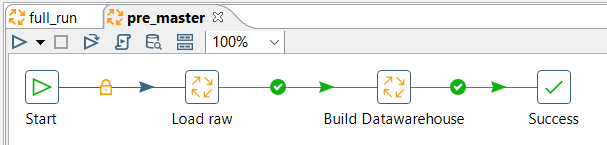
\includegraphics[width=0.7\linewidth]{Images/Pentaho/pre_master}
    }{
        \fbox{\begin{minipage}{0.7\linewidth}
            \centering
            \vspace{2cm}
            [IMAGE PLACEHOLDER]\\
            \texttt{Images/Pentaho/pre\_master.png}\\
            \vspace{2cm}
        \end{minipage}}
    }
    \caption{Luồng Pre-Master nạp dữ liệu gốc ban đầu}
    \label{fig:pentaho_pre_master}
\end{figure}

Luồng \textbf{Pre-Master} chịu trách nhiệm nạp toàn bộ lượng dữ liệu lịch sử khổng lồ từ tập dữ liệu ban đầu. Các bước thực thi bao gồm:
\begin{itemize}
    \item Đọc dữ liệu từ các file RAW CSV gốc.
    \item Nạp dữ liệu vào các bảng trong Staging Area (MSSQL).
    \item Chuyển và xử lý dữ liệu từ Staging Area sang Data Warehouse (PostgreSQL).
\end{itemize}

\subsubsection{Luồng Vận hành và Cập nhật Tự động (Master)}

\begin{figure}[H]
    \centering
    \IfFileExists{Images/Pentaho/master.png}{
        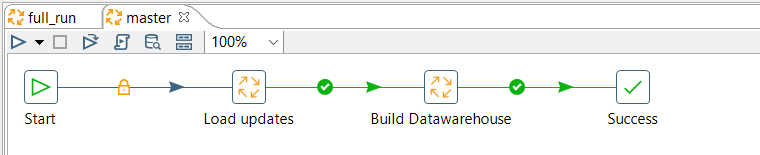
\includegraphics[width=0.9\linewidth]{Images/Pentaho/master}
    }{
        \fbox{\begin{minipage}{0.9\linewidth}
            \centering
            \vspace{2cm}
            [IMAGE PLACEHOLDER]\\
            \texttt{Images/Pentaho/master.png}\\
            \vspace{2cm}
        \end{minipage}}
    }
    \caption{Luồng Master xử lý và cập nhật dữ liệu thu thập mới}
    \label{fig:pentaho_master}
\end{figure}

Luồng \textbf{Master} là luồng được thiết lập để \textbf{lên lịch chạy tự động} trong hệ thống sản xuất. Chức năng chính của Master là:
\begin{itemize}
    \item Quét và xác thực sự hiện diện của dữ liệu mới được thu thập trong thư mục Landing. Quy trình xác thực Landing (Phase 00) được thực thi qua job \texttt{00\_validate\_landing.kjb} kết hợp các transforms rà soát thư mục con phân vùng. Hệ thống đối chiếu chéo với bảng kiểm toán \texttt{dbo.stg\_load\_audit} (nơi \texttt{status = 'success'}) nhằm xác định phân vùng cũ nhất chưa được xử lý, lưu vết đường dẫn vào biến Pentaho đồng thời bỏ qua các phân vùng đã hoàn tất nhằm bảo đảm tính lũy đẳng (idempotency).
    \item Nạp các dữ liệu mới này vào vùng đệm Staging.
    \item Chuyển từ Staging vào Data Warehouse để cập nhật dữ liệu mới nhất.
\end{itemize}

\subsection{Quy trình Tiền xử lý và Làm sạch Dữ liệu Chuyên sâu}

\subsubsection{Giai đoạn Nạp Dữ liệu vào Vùng đệm (Staging Load)}

Dữ liệu thô từ file CSV được đọc và đẩy vào các bảng đệm tạm thời tại MSSQL. Trong quy trình nạp thô (Phase 05 và Phase 10), hệ thống hỗ trợ các luồng chuyển đổi đọc thử nghiệm (optional preview) nhằm kiểm tra cấu trúc tệp (tiêu đề, số lượng cột) mà không thực hiện ghi nhận dữ liệu. Tiếp đó, 5 luồng chuyển đổi song song nạp dữ liệu thô vào các bảng đệm \texttt{dbo.stg\_players}, \texttt{stg\_history}, \texttt{stg\_reviews}, \texttt{stg\_purchased\_games}, và \texttt{stg\_private\_steamids} thuộc cơ sở dữ liệu \texttt{DW\_Staging}. Toàn bộ các trường thông tin tại vùng đệm đều được lưu trữ nguyên bản dưới định dạng chuỗi ký tự động \texttt{NVARCHAR(MAX)} nhằm tránh hao hụt thông tin đầu vào.

\begin{figure}[H]
    \centering
    \IfFileExists{Images/Pentaho/Stage_Raw.png}{
        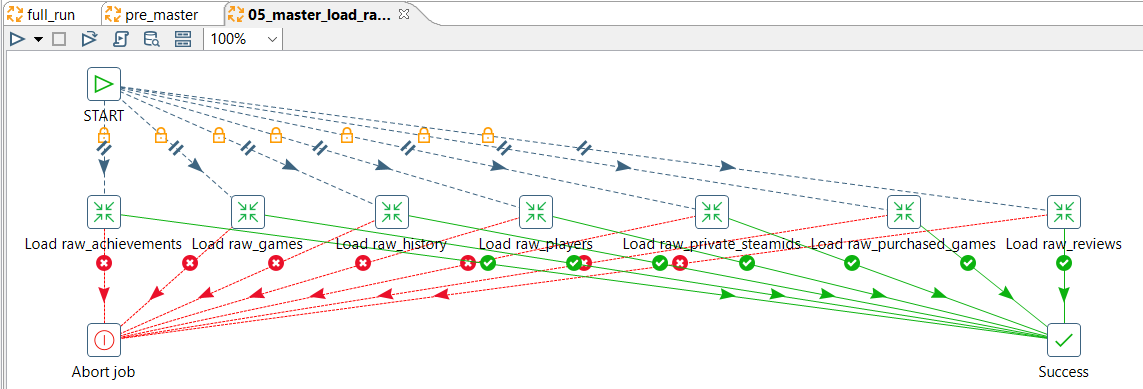
\includegraphics[width=0.7\linewidth]{Images/Pentaho/Stage_Raw}
    }{
        \fbox{\begin{minipage}{0.7\linewidth}
            \centering
            \vspace{2cm}
            [IMAGE PLACEHOLDER]\\
            \texttt{Images/Pentaho/Stage\_Raw.png}\\
            \vspace{2cm}
        \end{minipage}}
    }
    \caption{Quá trình nạp dữ liệu thô vào Staging}
    \label{fig:pentaho_stage_raw}
\end{figure}

\begin{figure}[H]
    \centering
    \IfFileExists{Images/Pentaho/Stage_Update.png}{
        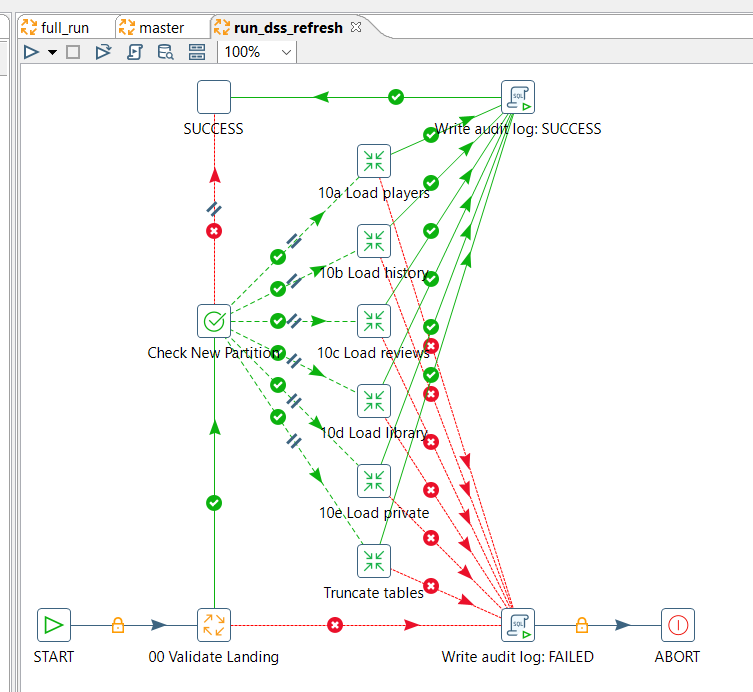
\includegraphics[width=0.7\linewidth]{Images/Pentaho/Stage_Update}
    }{
        \fbox{\begin{minipage}{0.7\linewidth}
            \centering
            \vspace{2cm}
            [IMAGE PLACEHOLDER]\\
            \texttt{Images/Pentaho/Stage\_Update.png}\\
            \vspace{2cm}
        \end{minipage}}
    }
    \caption{Quá trình nạp dữ liệu cập nhật vào Staging}
    \label{fig:pentaho_stage_update}
\end{figure}

\subsubsection{Giai đoạn Xây dựng Data Warehouse (Build DW)}

Đây là bước thực hiện các thao tác tiền xử lý dữ liệu của toàn bộ pipeline ETL.

\begin{figure}[H]
    \centering
    \IfFileExists{Images/Pentaho/Build_DW.png}{
        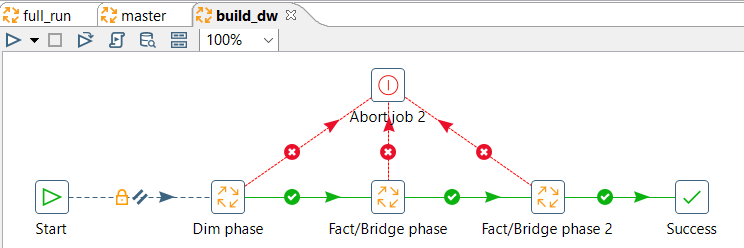
\includegraphics[width=0.7\linewidth]{Images/Pentaho/Build_DW}
    }{
        \fbox{\begin{minipage}{0.7\linewidth}
            \centering
            \vspace{2cm}
            [IMAGE PLACEHOLDER]\\
            \texttt{Images/Pentaho/Build\_DW.png}\\
            \vspace{2cm}
        \end{minipage}}
    }
    \caption{Quá trình tiền xử lý và xây dựng Data Warehouse}
    \label{fig:pentaho_build_dw}
\end{figure}

Trong bước Build DW (Phase 20), hệ thống thực hiện hàng loạt các quy tắc làm sạch và chuẩn hóa dữ liệu phức tạp. Dưới đây là 5 cơ chế tiền xử lý cốt lõi được áp dụng:

\begin{enumerate}
    \item \textbf{Khử trùng lặp dữ liệu (Deduplication):} Dữ liệu crawl về thường xuyên có sự trùng lặp. Ở tầng Staging, các truy vấn SQL sử dụng hàm cửa sổ \texttt{ROW\_NUMBER() OVER(PARTITION BY <pk> ORDER BY loaded\_at DESC)} để chỉ trích xuất phiên bản mới nhất của mỗi bản ghi (dựa trên thời điểm nạp) trước khi chuyển vào DW. 
    \item \textbf{Ép kiểu và chuẩn hóa định dạng (Type Casting):} Tất cả dữ liệu ở vùng Staging đều được lưu dưới dạng chuỗi \texttt{NVARCHAR(MAX)} để đảm bảo không bị mất dữ liệu trong quá trình nạp thô. Tại bước này, hệ thống sẽ thực hiện ép kiểu:
    \begin{itemize}
        \item \textbf{Ngày tháng:} Chuyển đổi chuỗi thành \texttt{Date} và \texttt{Timestamp} (ví dụ: ép kiểu \texttt{date\_acquired} sang định dạng \texttt{DD/MM/YYYY HH:mm} chuẩn UTC).
        \item \textbf{Số học:} Ép kiểu các trường tương tác của review (\texttt{helpful, funny, awards}) sang dạng số nguyên.
        \item \textbf{Văn bản:} Giữ nguyên định dạng chuỗi dài để bảo toàn các ký tự UTF-8 phức tạp (như review tiếng Trung, Nga, Emoji). Cụ thể, trường văn bản đánh giá được ấn định kích thước giới hạn tiệm cận \texttt{1073741823} byte nhằm ánh xạ chính xác vào trường \texttt{TEXT} trên hệ quản trị đích.
    \end{itemize}
    \item \textbf{Bóc tách và định hình lại cấu trúc (Data Reshaping):} Cột \texttt{library} của mỗi người dùng ban đầu được lưu dưới dạng một mảng JSON nguyên khối (VD: \texttt{[\{"appid":730,"playtime\_mins":500\}]}). Dữ liệu này được đẩy vào bảng trung gian \texttt{stg\_library\_temp}, sau đó sử dụng Common Table Expression (CTE) kết hợp các hàm xử lý JSON của PostgreSQL để giải nén (unnest) và trải phẳng thành nhiều bản ghi riêng biệt \texttt{(playerid, appid, playtime\_mins)} trong bảng \texttt{fact\_library}. Quá trình tải trung gian áp dụng triệt để chiến lược \texttt{<truncate>Y</truncate>} làm sạch bảng tạm nhằm tối ưu dung lượng.
    \item \textbf{Bảo đảm toàn vẹn tham chiếu qua Trigger (Referential Integrity Fallback):} Do tính chất không đồng bộ của quá trình thu thập, đôi khi một bản ghi Fact có thể trỏ tới một chiều (Dimension) chưa tồn tại. Hệ thống PostgreSQL DW sử dụng các trigger \texttt{BEFORE INSERT} để kiểm soát luồng dữ liệu:
    \begin{itemize}
        \item \textbf{Xóa bỏ bản ghi lỗi (Hard-reject):} Nếu Fact trỏ tới một \texttt{playerid} hoàn toàn không tồn tại, dòng dữ liệu đó bị xóa bỏ vì là dữ liệu rác. Cụ thể, các chốt chặn này thực thi lệnh \texttt{RETURN NULL} để gạch bỏ trong im lặng khi khóa ngoại bắt buộc khuyết thiếu hoặc phát sinh vi phạm trùng lặp khóa chính.
        \item \textbf{Tự động sinh dữ liệu ảo (Auto-stubbing):} Nếu một game hoặc một thành tựu chưa tồn tại trong dimension nhưng lại xuất hiện trong các bảng sự kiện (Fact), trigger sẽ tự động trích xuất thông tin (như \texttt{gameid} từ prefix của \texttt{achievementid}) và tạo dòng dữ liệu tạm (stub) với tiêu đề \texttt{"Unknown (auto-stub)"}. Cơ chế này bảo đảm không có bản ghi nào bị mất mát do lỗi tham chiếu, tránh làm sai lệch các chỉ số đặc trưng (feature matrix) sau này.
    \end{itemize}
    \item \textbf{Bổ trợ Tính toán và Ánh xạ Địa lý:} Hệ thống tích hợp hàm \texttt{calculate\_shannon\_entropy} trực tiếp tại tầng Database để tính toán độ hỗn loạn thời gian chơi, đồng thời duy trì bảng tham chiếu \texttt{dim\_country\_utc\_offset} để chuẩn hóa múi giờ cho 54 quốc gia trọng điểm dựa trên mã ISO 3166-1.
    \item \textbf{Tối ưu hóa Băng thông và Xử lý Ngoại lệ:} Để đáp ứng lưu lượng tải lớn, các bước chuyển đổi quan trọng được thiết lập cơ chế thực thi bản sao song song (parallelism): luồng nạp bảng chiều \texttt{dim\_player} kích hoạt đồng thời 2 bản sao, trong khi luồng nạp sự kiện \texttt{fact\_achievement\_unlock} phân mảnh qua 4 bản sao thực thi. Song song đó, quy mô gói nạp (commit size) được tinh chỉnh động: áp dụng mức 20.000 dòng cho các bảng chiều và bảng tạm thư viện, đồng thời thu hẹp xuống 100 dòng cho các bảng sự kiện tích hợp trigger nhằm bảo đảm tính ổn định. Các bản ghi phát sinh lỗi ép kiểu hoặc xung đột chèn dữ liệu được cơ chế định tuyến lỗi (step error routing) tự động cô lập và xuất ra tệp nhật ký \texttt{err\_log.csv} phục vụ rà soát.
\end{enumerate}

Để đảm bảo tính toàn vẹn cấu trúc và thỏa mãn các ràng buộc khóa ngoại (key constraints), quá trình Build DW bắt buộc phải được thực hiện qua 3 giai đoạn tuần tự:
\begin{enumerate}
    \item \textbf{Phase 1:} Xây dựng các bảng Dimension (Dim Game, Dim Player).
    \item \textbf{Phase 2:} Xây dựng các bảng Fact cấp một (Fact Achievement, Private SteamID, Fact Library, Fact Review).
    \item \textbf{Phase 3:} Xây dựng các bảng Fact cấp hai (phụ thuộc vào dữ liệu của các bảng đã được nạp ở giai đoạn trước, bao gồm: Fact Achievement Unlock).
\end{enumerate}

\subsubsection{Tổng hợp Quy tắc Làm sạch theo Từng bảng (Per-Table Cleaning Inventory)}

Dưới đây là chi tiết các cơ chế tiền xử lý được áp dụng cụ thể cho từng bảng dữ liệu khi chuyển từ Staging sang Data Warehouse:

\begin{itemize}
    \item \textbf{Tất cả các bảng (All Tables):}
    \begin{itemize}
        \item \textbf{Theo dõi thời gian (Temporal tracking):} Gắn nhãn thời gian nạp \texttt{loaded\_at DEFAULT SYSUTCDATETIME()} tại tầng Staging.
        \item \textbf{Khử trùng lặp (Deduplication):} Sử dụng \texttt{ROW\_NUMBER() OVER(PARTITION BY <pk> ORDER BY loaded\_at DESC) WHERE rn=1} trong câu truy vấn SQL lấy dữ liệu, kết hợp với các Trigger \texttt{BEFORE INSERT} kiểm tra khóa chính (PK) ở tầng Database để ngăn chặn chèn trùng lặp.
    \end{itemize}

    \item \textbf{Bảng Người Chơi (Dim Player):}
    \begin{itemize}
        \item \textbf{Ép kiểu (Type casting):} Chuyển chuỗi \texttt{created} sang định dạng \texttt{Timestamp} (áp dụng chuỗi định dạng tham chiếu \texttt{\%Y-\%m-\%d \%H:\%M:\%S}).
        \item \textbf{Đánh dấu quyền riêng tư (Privacy flagging):} Cập nhật cờ \texttt{is\_private = TRUE} dựa trên danh sách từ bảng Private SteamIDs.
    \end{itemize}

    \item \textbf{Bảng Lịch Sử Thành Tựu (Fact Achievement Unlock):}
    \begin{itemize}
        \item \textbf{Ép kiểu (Type casting):} Chuyển \texttt{date\_acquired} sang định dạng \texttt{Timestamp} (UTC).
        \item \textbf{Xử lý tham chiếu vắng mặt (FK stub creation):} Nếu một thành tựu (\texttt{achievementid}) chưa được ghi nhận trong bảng \texttt{Fact Achievement}, trigger sẽ tự động trích xuất \texttt{gameid} từ tiền tố của \texttt{achievementid} (VD: từ "730\_WINS\_1" lấy ra "730"), sau đó tự động tạo dòng dữ liệu tạm (stub) cho cả \texttt{Dim Game} và \texttt{Fact Achievement} trước khi nạp lịch sử này.
        \item \textbf{Lọc giá trị Null (Null rejection):} Loại bỏ hoàn toàn các bản ghi có \texttt{playerid} hoặc \texttt{achievementid} bị rỗng (NULL).
    \end{itemize}

    \item \textbf{Bảng Đánh Giá (Fact Review):}
    \begin{itemize}
        \item \textbf{Ép kiểu (Type casting):} Chuyển \texttt{helpful, funny, awards} sang \texttt{Integer}; chuyển \texttt{posted} sang \texttt{Date}.
        \item \textbf{Tham chiếu mặc định (FK fallback):} Nếu \texttt{gameid} không tồn tại trong \texttt{Dim Game}, hệ thống tự động gán về giá trị mặc định \texttt{'-1'}.
        \item \textbf{Lọc dữ liệu rác (Player validation):} Xóa bỏ bản ghi nếu \texttt{playerid} không tồn tại trong \texttt{Dim Player}.
    \end{itemize}

    \item \textbf{Bảng Thư Viện Trò Chơi (Fact Library):}
    \begin{itemize}
        \item \textbf{Giải nén JSON (JSON explosion):} Biến đổi cột \texttt{library} từ mảng JSON thành nhiều hàng \texttt{(playerid, appid, playtime\_mins)} thông qua truy vấn CTE.
        \item \textbf{Xử lý Null (Null handling):} Các bản ghi bị thiếu thông tin giờ chơi (\texttt{playtime\_mins} mang giá trị NULL hoặc 'NaN') được chuẩn hóa về \texttt{0} ngay tại tầng Database thông qua hàm \texttt{COALESCE} trong Trigger. Việc này bảo đảm tính toàn vẹn toán học cho các bước tổng hợp đặc trưng sau này.
        \item \textbf{Xử lý tham chiếu vắng mặt (FK stub creation):} Nếu \texttt{appid} chưa có trong \texttt{Dim Game}, trigger tự động thực hiện \texttt{INSERT} một bản ghi stub mới vào bảng chiều với tiêu đề \texttt{'Unknown (auto-stub)'}.
    \end{itemize}

    \item \textbf{Bảng Trò Chơi (Dim Game):}
    \begin{itemize}
        \item \textbf{Ép kiểu (Type casting):} Chuyển \texttt{release\_date} sang định dạng \texttt{Date}.
    \end{itemize}

    \item \textbf{Bảng Thành Tựu (Fact Achievement):}
    \begin{itemize}
        \item \textbf{Tham chiếu mặc định (FK fallback):} Tự động gán \texttt{gameid = '-1'} nếu trò chơi tương ứng chưa được ghi nhận.
    \end{itemize}
\end{itemize}
\newpage
\chapter{Feature Engineering}

% TODO: Feature Engineering
\newpage
\chapter{Xây Dá»±ng Mô Hình (Model Selection, Training \& Tuning)}

\section{Tổng Quan}
Hệ thống sử dụng hai mô hình machine learning chính: \textbf{XGBoost} và \textbf{IsolationForest}, được kết hợp trong một ensemble để tăng độ chính xác và độ tin cậy của phát hiện bot.

\section{Xử Lý Dữ Liệu Trước Training}

\subsection{Đường Dẫn A: IsolationForest}

\subsubsection{BÆ°á»›c 1: Log Transform}
Để tăng ổn định của đường dẫn trong IsolationForest, hệ thống áp dụng log-transform cho 9 đặc trưng có phân phối nặng về đuôi (heavy-tailed):

\begin{equation}
\text{feature\_transformed} = \log_1p(\text{clip}(x, \min=0))
\end{equation}

\textbf{Lý do}: Các đặc trưng như \texttt{max\_achievements\_per\_day}, \texttt{total\_achievements} có phạm vi 6+ bậc độ lớn. Random split không đều không đại diện đủ cho mật độ dữ liệu thực. Log transform cân bằng lại phạm vi.

\subsubsection{BÆ°á»›c 2: Preprocessing}
\begin{itemize}
    \item \texttt{SimpleImputer(strategy='median')}: Điền giá trị thiếu bằng median
    \item \texttt{StandardScaler}: Chuẩn hóa dữ liệu về trung bình = 0, độ lệch chuẩn = 1
    \item Output: DataFrame $X_{IF}$ được lưu sạch
    \item Lưu trữ: File \texttt{preprocessor.pkl} chứa pipeline preprocessing
\end{itemize}

\subsection{Đường Dẫn B: XGBoost}

\textbf{Chiến lược}: Sử dụng $X_{raw}$ trực tiếp (không impute, không scale)

\textbf{Lý do}:
\begin{itemize}
    \item XGBoost xử lý NaN natively thông qua sparsity-aware split finding
    \item NaN trong review features (người dùng không viết đánh giá) là \textbf{tín hiệu thực sự}, không phải gap cần điền
    \item XGBoost bất biến với monotonic transform → log-transform không có tác dụng
\end{itemize}

\section{Model A: IsolationForest}

\subsection{Tuning}
\begin{itemize}
    \item Phương pháp: Grid search trên siêu tham số
    \item Objective: Tối đa hóa ROC-AUC so với $y_{heuristic}$ (nhãn sử dụng heuristic rule)
    \item Output: $best\_if\_params$ (best hyperparameters)
\end{itemize}

\subsection{Training}
\begin{itemize}
    \item Sử dụng $X_{IF}$ (log-transformed + scaled)
    \item Áp dụng $best\_if\_params$
    \item Output: Mô hình \texttt{best\_if.pkl}
    \item Metric: ROC-AUC để đánh giá chất lượng
\end{itemize}

\section{Model B: XGBoost (Semi-Supervised)}

\subsection{Chuẩn Bị Dữ Liệu}
Training chỉ diễn ra trên \textbf{confident subset}:
\begin{equation}
\text{confident\_mask} = (y_{heuristic} == 1) \text{ OR } (y_{normal} == 1)
\end{equation}

Các tài khoản trong "grey area" (không bot, không chắc chắn normal) được loại bỏ để tăng chất lượng training signal.

\subsection{Tuning}

\subsubsection{Xử Lý Class Imbalance}
\begin{equation}
\text{scale\_pos\_weight} = \frac{\text{negative\_count}}{\text{positive\_count}}
\end{equation}

Tỷ lệ này giúp XGBoost cân bằng chi phí lỗi giữa class bot và normal.

\subsubsection{Tìm Siêu Tham Số Tối Ưu}
\begin{itemize}
    \item Phương pháp: \texttt{RandomizedSearchCV}
    \item Số lần tìm kiếm: $n\_iter = 50$
    \item Cross-validation: 5-fold
    \item Metric: \textbf{PR-AUC (Precision-Recall AUC)} — ưu tiên cho dữ liệu imbalanced
    \item Output: $best\_xgb$ (best model), lưu vào \texttt{best\_xgb.pkl}
\end{itemize}

\subsection{Training \& Prediction}
\begin{itemize}
    \item Training data: Confident subset của $X_{raw}$
    \item Prediction: Chạy \texttt{predict\_proba()} trên \textbf{toàn bộ} $X_{raw}$ (không chỉ training subset)
    \item Output: Probability scores (0–1) cho tất cả tài khoản
    \item Lưu trữ: \texttt{xgb\_tuning\_results.csv} chứa chi tiết các lần tìm kiếm
\end{itemize}

\section{Xây Dựng Ensemble}

\subsection{Chiến Lược}
Kết hợp hai mô hình để tận dụng điểm mạnh của từng mô hình:

\subsubsection{BÆ°á»›c 1: Rank Percentile}
\begin{itemize}
    \item Tính percentile rank của IF scores: $if\_pct = \text{percentileofscore}(if\_scores) \in [0, 100]$
    \item Tính percentile rank của XGBoost probabilities: $xgb\_pct = \text{percentileofscore}(xgb\_proba) \in [0, 100]$
\end{itemize}

\subsubsection{BÆ°á»›c 2: Composite Score}
\begin{equation}
\text{composite} = 0.70 \times xgb\_pct + 0.30 \times if\_pct
\end{equation}

Trọng số 70:30 ưu tiên XGBoost (supervised signal mạnh hơn) nhưng vẫn giữ IsolationForest để bắt unsupervised anomalies.

\subsubsection{Bước 3: Quyết Định Anomaly}
\begin{equation}
is\_anomaly = \text{composite} \geq 85
\end{equation}

Ngưỡng 85 là điểm cắt để phân loại tài khoản là bot hay normal.

\subsection{Tuning Trọng Số Ensemble (Optional)}
Bước phân tích thêm để tối ưu trọng số:

\begin{itemize}
    \item Sweep $xgb\_weight$ từ 0.0 → 1.0 (bước 0.05)
    \item Tại mỗi điểm, tính 3 metrics:
    \begin{itemize}
        \item \textbf{Precision@100}: Độ chính xác trong top-100 flagged
        \item \textbf{PR-AUC}: Area under precision-recall curve
        \item \textbf{High\_Conflict\_Cases (HCC)}: Số tài khoản có mô hình không đồng ý
    \end{itemize}
    \item Tìm "optimal sweet spot": argmax Precision@100 trong tập HCC ≥ median(HCC)
    \item Output: \texttt{ensemble\_weight\_metrics.csv}, \texttt{plots/ensemble\_weight\_tuning.png}
\end{itemize}

\section{Lưu Trữ Mô Hình \& Siêu Tham Số}

\subsection{File Lưu Trữ}
\begin{table}[h]
\centering
\begin{tabular}{|l|l|}
\hline
\textbf{Tên File} & \textbf{Nội Dung} \\
\hline
\texttt{best\_if.pkl} & Mô hình IsolationForest đã train \\
\texttt{best\_xgb.pkl} & Mô hình XGBoost đã train \\
\texttt{preprocessor.pkl} & Pipeline preprocessing (SimpleImputer + StandardScaler) \\
\texttt{xgb\_tuning\_results.csv} & Chi tiết 50 lần tìm kiếm XGBoost (siêu tham số + metric) \\
\texttt{ensemble\_weight\_metrics.csv} & Kết quả tuning trọng số ensemble \\
\hline
\end{tabular}
\end{table}

\subsection{Thông Tin Siêu Tham Số}
\begin{itemize}
    \item \textbf{IsolationForest}: Stored in \texttt{best\_if.pkl}
    \begin{itemize}
        \item Các siêu tham số như \texttt{n\_estimators}, \texttt{contamination}, \texttt{random\_state}, v.v.
    \end{itemize}
    \item \textbf{XGBoost}: Stored in \texttt{best\_xgb.pkl}
    \begin{itemize}
        \item Các siêu tham số như \texttt{max\_depth}, \texttt{learning\_rate}, \texttt{subsample}, \texttt{scale\_pos\_weight}, v.v.
        \item Chi tiết tuning process lưu trong \texttt{xgb\_tuning\_results.csv}
    \end{itemize}
    \item \textbf{Ensemble Weights}: Mặc định 70:30 (XGBoost:IsolationForest), có thể điều chỉnh dựa trên \texttt{ensemble\_weight\_metrics.csv}
\end{itemize}

\section{Tóm Tắt}
Hệ thống training gồm 3 giai đoạn: (1) preprocessing riêng biệt cho IF vs XGBoost, (2) tuning siêu tham số cho từng mô hình độc lập, (3) kết hợp trong ensemble weighted. Tất cả mô hình, preprocessor, và kết quả tuning được lưu trữ cho tái sử dụng và truy vết.

\newpage
\chapter{Dự Báo Tương Lai \& Ứng Dụng Mô Hình}

\section{Tổng Quan}
Sau khi training, mô hình ensemble được sử dụng để:
\begin{enumerate}
    \item Dự báo trên toàn bộ dữ liệu (inference)
    \item Xác định tài khoản bot với độ tin cậy cao
    \item Tạo mẫu để human review và cải thiện liên tục (Active Learning)
    \item Đánh giá chất lượng mô hình thông qua các metrics toàn diện
\end{enumerate}

\section{Inference \& Dự Báo Bot}

\subsection{Quy Trình}
\begin{enumerate}
    \item Load trained models: \texttt{best\_if.pkl}, \texttt{best\_xgb.pkl}, \texttt{preprocessor.pkl}
    \item Xử lý feature matrix $X_{\text{raw}}$:
    \begin{itemize}
        \item IF path: Log-transform → Preprocess (SimpleImputer + StandardScaler)
        \item XGBoost path: Sử dụng $X_{\text{raw}}$ trực tiếp (không transform)
    \end{itemize}
    \item Prediction:
    \begin{itemize}
        \item $if\_scores = best\_if.decision\_function(X\_{IF})$
        \item $xgb\_proba = best\_xgb.predict\_proba(X\_{raw})[:, 1]$ (probability of bot class)
    \end{itemize}
    \item Ensemble:
    \begin{itemize}
        \item Convert sang percentile ranks: $if\_pct$, $xgb\_pct \in [0, 100]$

        \item Composite: $\text{composite} = 0.70 \times xgb\_pct + 0.30 \times if\_pct$
        \item Prediction: $is\_anomaly = \text{composite} \geq 85$
    \end{itemize}
\end{enumerate}

\subsection{Output}
\begin{itemize}
    \item Danh sách tài khoản được flagged là bot (là những tài khoản có $is\_anomaly = 1$)
    \item Composite score cho mỗi tài khoản (độ tin cậy 0–100)
    \item XGBoost probability score và IF anomaly score riêng lẻ (để debug \& análysis)
\end{itemize}

\section{Active Learning Loop}

\subsection{Xác Định Mẫu Để Review}

\textbf{Mục tiêu}: Tìm các trường hợp "conflict" để cải thiện mô hình

\textbf{Điều kiện}:
\begin{equation}
\text{conflict} = (\text{composite} \geq 85) \text{ AND } (\text{heuristic\_bot} == 0)
\end{equation}

Những tài khoản này là:
\begin{itemize}
    \item Mô hình học máy dự báo là BOT ($\text{composite} \geq 85$)

    \item Nhưng heuristic rule không phát hiện là bot
    \item Có thể là false positive hoặc heuristic bỏ sót
\end{itemize}

\subsection{Tạo Mẫu Để Review}

Module \texttt{active\_learning.py} - Function \texttt{generate\_review\_sample()}:

\begin{enumerate}
    \item Lọc: Chỉ lấy conflict cases
    \item Sắp xếp: Sort by $\text{composite\_score}$ descending (highest suspicion first)
    \item Chọn mẫu: Top 50 conflict cases
    \item Merge: Kết hợp với feature matrix → tạo context đầy đủ cho reviewer
    \item Lưu: Output file \texttt{outputs/to\_review.csv}
\end{enumerate}

\subsection{Human Labeling \& Feedback Loop}

\begin{enumerate}
    \item Human reviewer mở \texttt{to\_review.csv}
    \item Cho mỗi tài khoản, gán nhãn: $human\_label \in \{0, 1\}$
    \begin{itemize}
        \item 1 = Bot (mô hình đúng)
        \item 0 = Normal (mô hình sai)
        \item Blank = Không chắc chắn (bỏ qua)
    \end{itemize}
    \item Lưu file đã gán nhãn: \texttt{data/reviewed.csv}
    \item Re-run pipeline: Mô hình được train lại với:
    \begin{itemize}
        \item $integrate\_human\_labels()$ override heuristic labels bằng human labels (giai đoạn preprocessing)
        \item Confident subset được cải thiện → chất lượng training signal tăng
    \end{itemize}
\end{enumerate}

\subsection{Integration Logic}

Module \texttt{features.py} - Function \texttt{integrate\_human\_labels()}:

\begin{itemize}
    \item Đọc \texttt{data/reviewed.csv}
    \item Với mỗi row có hợp lệ human\_label (0 hoặc 1):
    \begin{itemize}
        \item Override $y\_{heuristic}[playerid]$ và/hoặc $y\_{normal}[playerid]$ bằng human label
    \end{itemize}
    \item Bỏ qua rows với blank labels
    \item HITL (Human-in-the-Loop) loop từ pipeline phục vụ cải thiện liên tục
\end{itemize}

\section{Evaluation \& Model Quality Assessment}

Module \texttt{evaluate.py}:

\subsection{So Sánh Các Mô Hình}

Function \texttt{\_model\_comparison()}:

Tính các metrics cho 3 mô hình: XGBoost, IsolationForest, Ensemble

\begin{itemize}
    \item \textbf{ROC-AUC}: Diện tích dưới đường cong ROC (tolerance mức độ trade-off giữa TPR \& FPR)
    \item \textbf{PR-AUC}: Diện tích dưới đường cong Precision-Recall (phù hợp với dữ liệu imbalanced)
    \item \textbf{Flagged Rate (\%)}: Tỷ lệ tài khoản được phân loại là bot
    \item \textbf{Precision@100/500/1000}: Độ chính xác trong top-N flagged accounts
\end{itemize}

Output: \texttt{model\_comparison.csv}

\subsection{Đánh Giá Chi Tiết XGBoost}

\begin{figure}[H]
    \centering
    \IfFileExists{Images/Slide/img151.jpg}{
        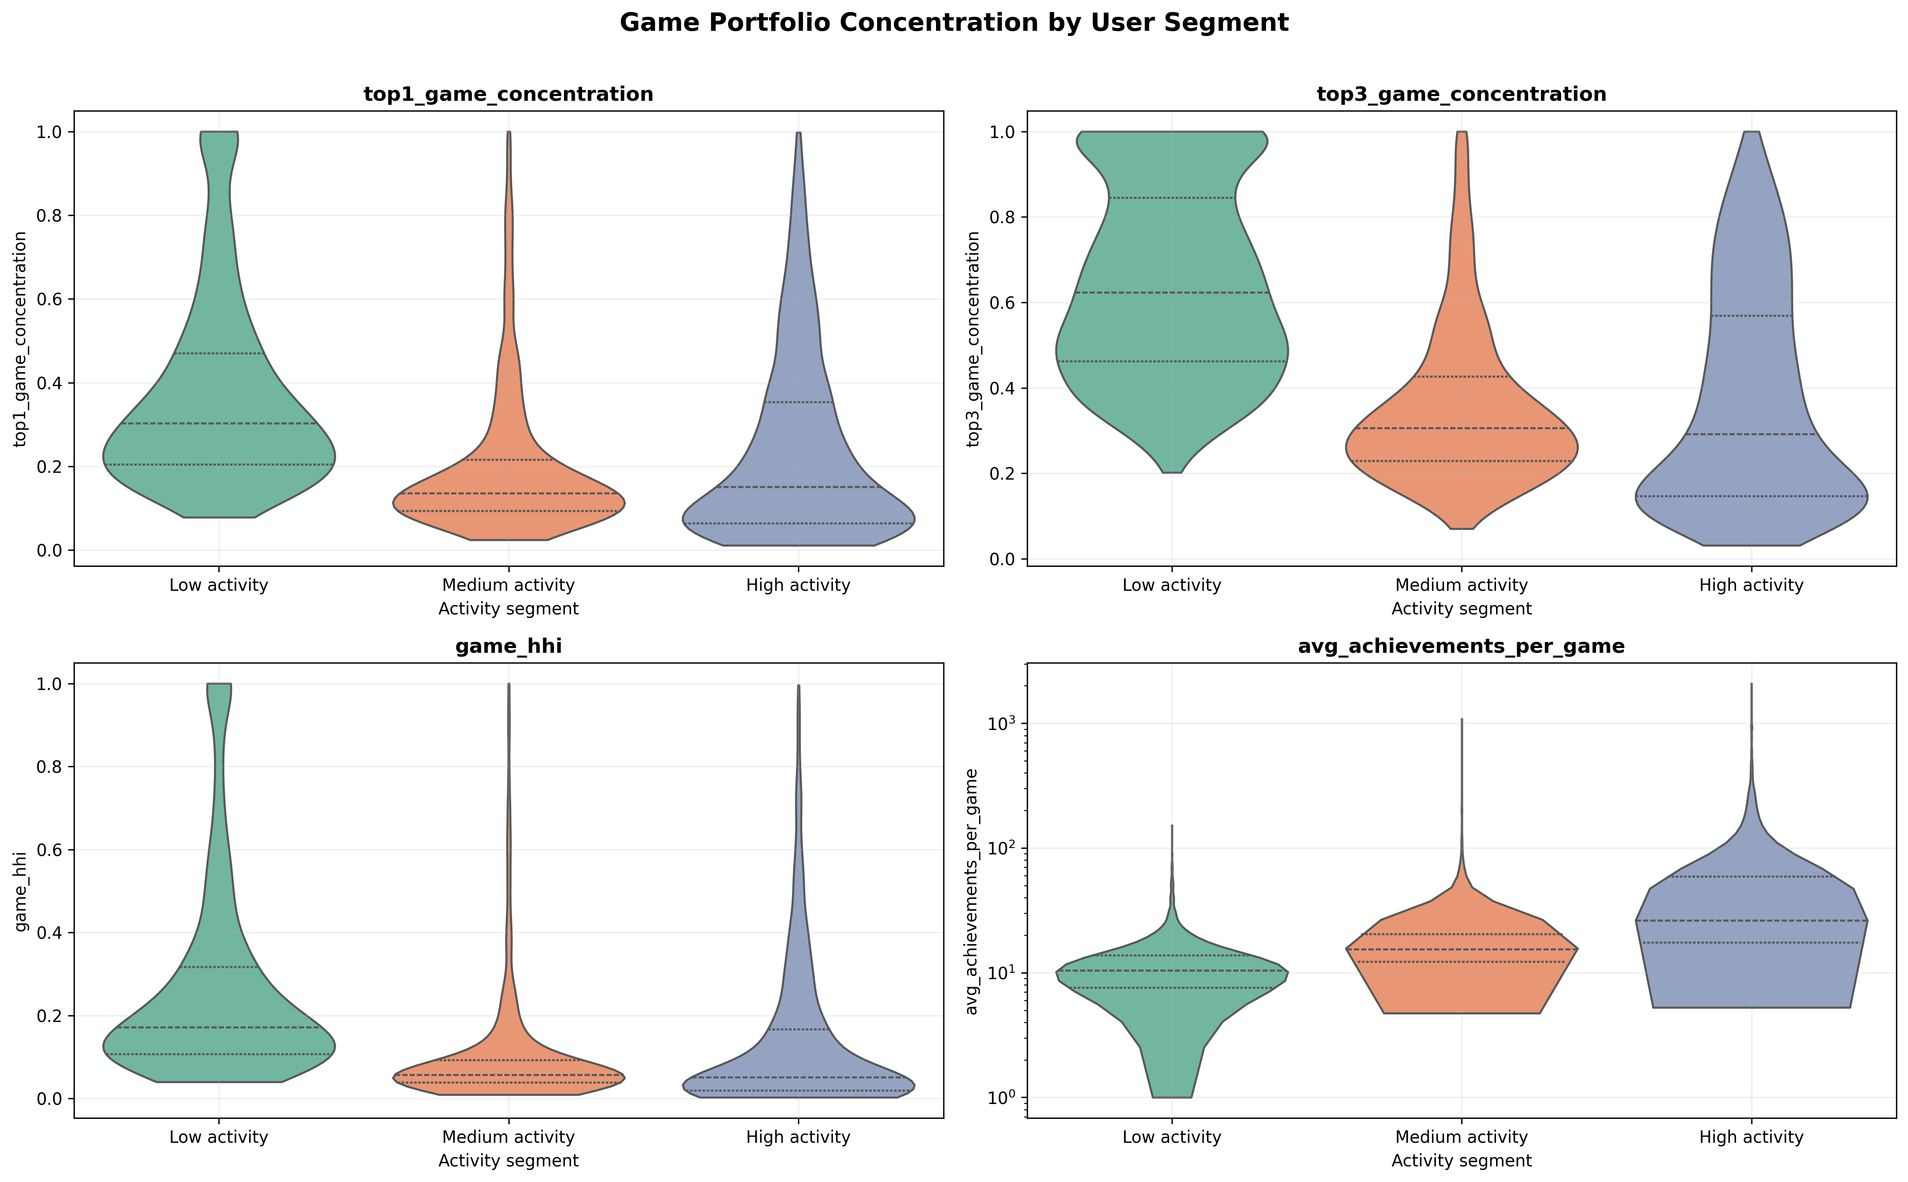
\includegraphics[width=0.7\linewidth]{Images/Slide/img151}
    }{
        \fbox{\begin{minipage}{0.7\linewidth}
            \centering
            \vspace{2cm}
            [IMAGE PLACEHOLDER]\\
            \texttt{Images/Slide/img151.jpg}\\
            \vspace{2cm}
        \end{minipage}}
    }
    \caption{Tầm quan trọng của các đặc trưng trong mô hình XGBoost}
    \label{fig:xgb_importance}
\end{figure}


Function \texttt{\_evaluate\_xgboost()}:

\begin{itemize}
    \item \textbf{PR-AUC}: 0.7252
    \item \textbf{ROC-AUC}: 0.9050
    \item \textbf{Optimal Threshold}: 0.9982 (F1-score tối ưu)
    \item \textbf{Classification Report (Bot class)}: Precision: 0.91, Recall: 0.66, F1-Score: 0.76
    \item Output plots:
    \begin{itemize}
        \item \texttt{xgb\_pr\_curve.png}: Đường cong Precision-Recall
        \item \texttt{xgb\_feature\_importance.png}: Biểu đồ tầm quan trọng đặc trưng
    \end{itemize}
\end{itemize}


\subsection{Phân Tích So Sánh Đặc Trưng}

\begin{itemize}
    \item So sánh: Top-50 flagged accounts vs Normal accounts
    \item Tính: Mean của mỗi đặc trưng trong 2 nhóm
    \item Output: \texttt{top50\_flagged\_profiles.csv} — profile trung bình của bot vs normal
    \item Giúp hiểu thành phần nào của feature matrix là discriminative nhất
\end{itemize}

\subsection{Phân Tích Khả Năng Giải Thích SHAP}

Giải thích độ đóng góp của từng đặc trưng đối với từng dự báo:

\begin{enumerate}
    \item \textbf{Sampling}: Chọn ngẫu nhiên 5000 hàng từ $X_{\text{raw}}$ (giữ thang đo gốc để dễ giải thích).
    \item \textbf{SHAP Calculation}: Tính SHAP values thông qua tính năng \texttt{pred\_contribs} của XGBoost.
    \item \textbf{Visualization}: Xuất các biểu đồ Summary, Waterfall và Scatter để phân tích tác động cục bộ và toàn cục.
\end{enumerate}

\begin{figure}[H]
    \centering
    \IfFileExists{Images/Slide/img156.jpg}{
        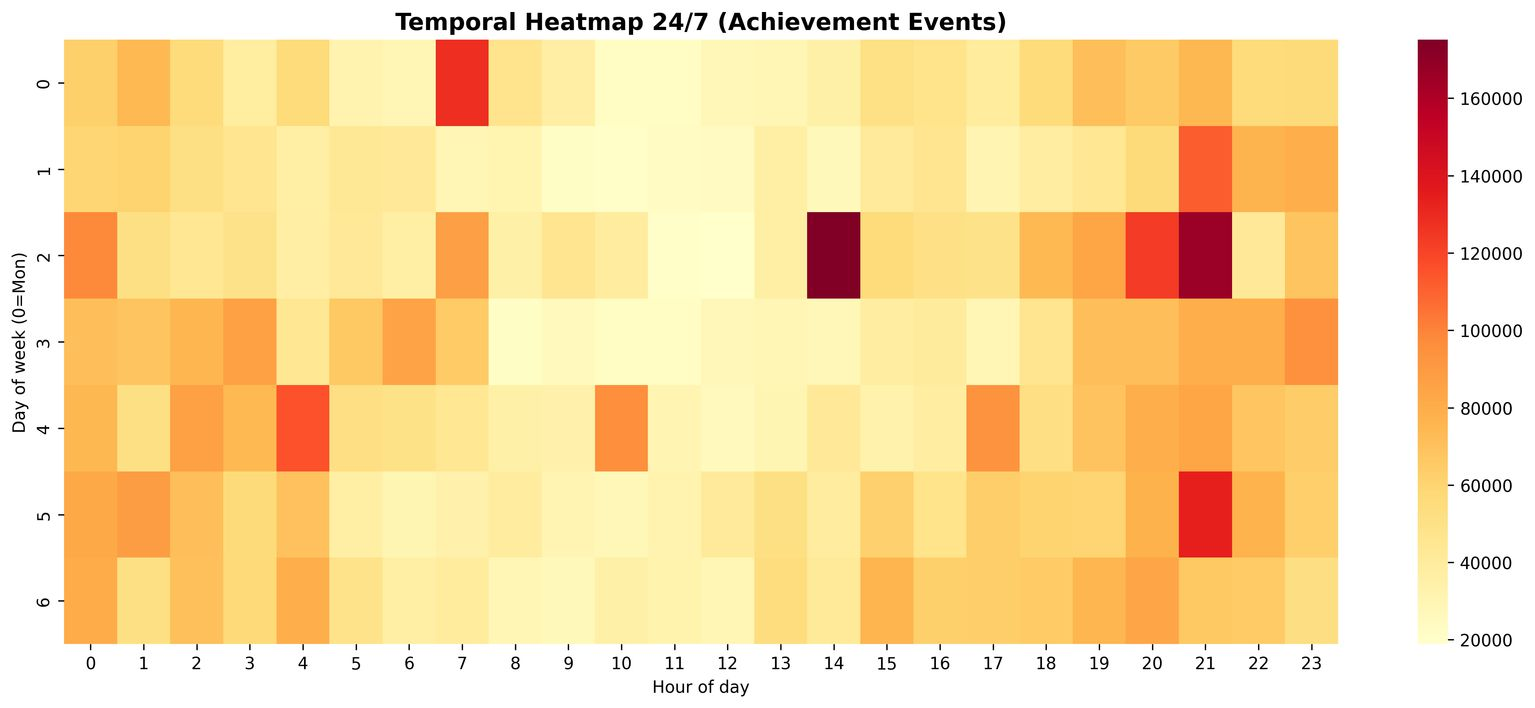
\includegraphics[width=0.7\linewidth]{Images/Slide/img156}
    }{
        \fbox{\begin{minipage}{0.7\linewidth}
            \centering
            \vspace{2cm}
            [IMAGE PLACEHOLDER]\\
            \texttt{Images/Slide/img156.jpg}\\
            \vspace{2cm}
        \end{minipage}}
    }
    \caption{Biểu đồ SHAP scatter thể hiện tác động của các giá trị đặc trưng}
    \label{fig:shap_scatter}
\end{figure}


\begin{figure}[H]
    \centering
    \IfFileExists{Images/Slide/img157.jpg}{
        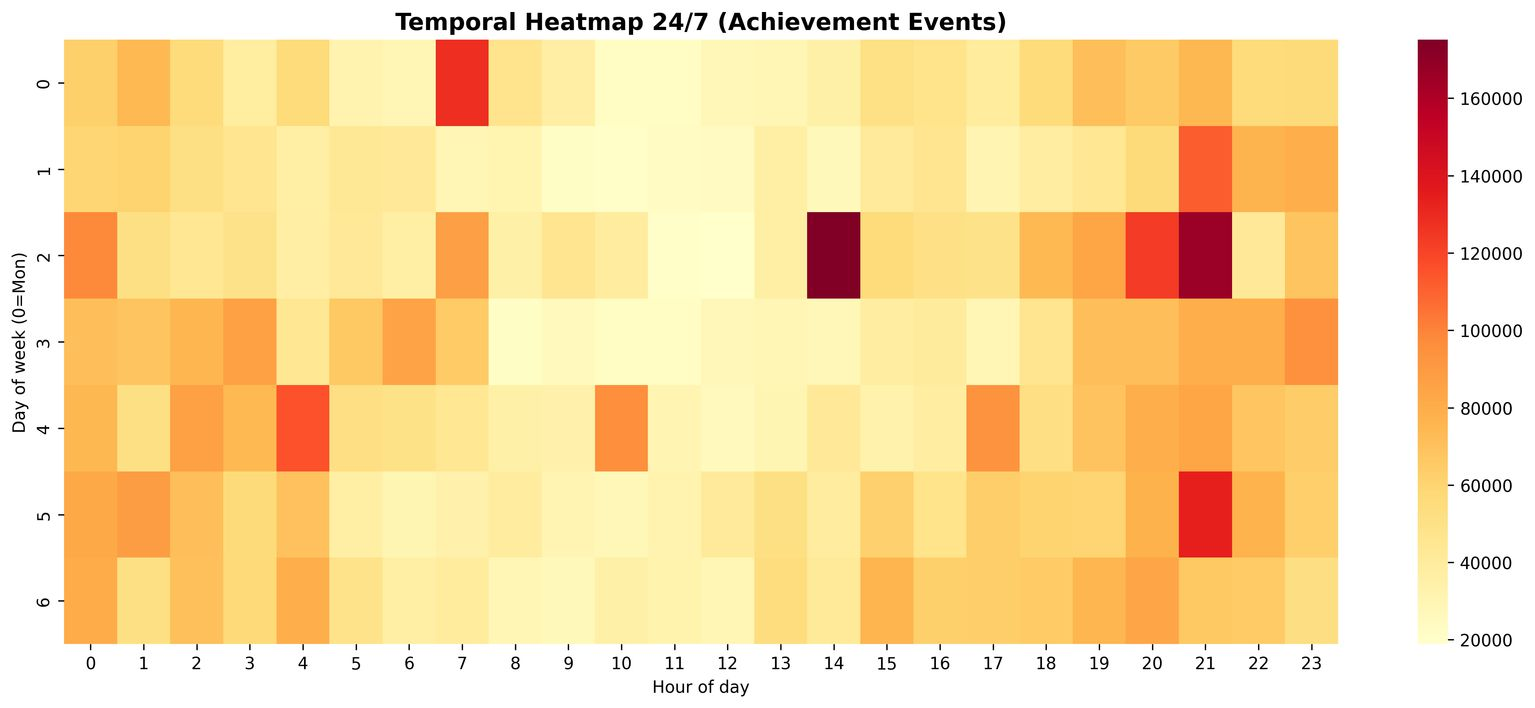
\includegraphics[width=0.7\linewidth]{Images/Slide/img157}
    }{
        \fbox{\begin{minipage}{0.7\linewidth}
            \centering
            \vspace{2cm}
            [IMAGE PLACEHOLDER]\\
            \texttt{Images/Slide/img157.jpg}\\
            \vspace{2cm}
        \end{minipage}}
    }
    \caption{Biểu đồ SHAP waterfall giải thích cho một trường hợp cụ thể}
    \label{fig:shap_waterfall}
\end{figure}


\section{Hệ Thống Dashboard BI}

Hệ thống cung cấp giao diện trực quan để theo dõi và phân tích các tài khoản bất thường.

\subsection{Giao Diện Tìm Kiếm và Truy Vấn}
Người dùng có thể tìm kiếm theo Steam ID hoặc tải lên danh sách file CSV/TXT.

\begin{figure}[H]
    \centering
    \IfFileExists{Images/Slide/img162.jpg}{
        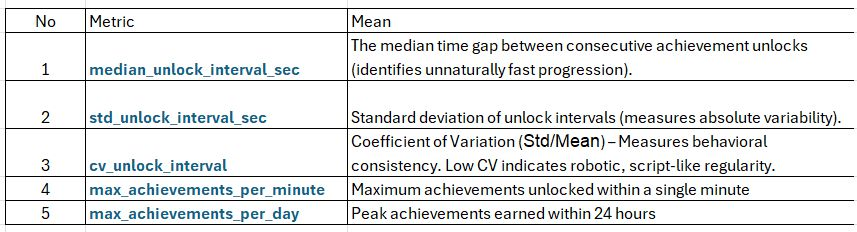
\includegraphics[width=0.7\linewidth]{Images/Slide/img162}
    }{
        \fbox{\begin{minipage}{0.7\linewidth}
            \centering
            \vspace{2cm}
            [IMAGE PLACEHOLDER]\\
            \texttt{Images/Slide/img162.jpg}\\
            \vspace{2cm}
        \end{minipage}}
    }
    \caption{Giao diện tìm kiếm tài khoản trên Dashboard}
    \label{fig:dash_search}
\end{figure}


\subsection{Chi Tiết Hành Vi và So Sánh Baseline}
Hệ thống hiển thị các chỉ số hành vi chi tiết so với mức trung bình của cộng đồng.

\begin{figure}[H]
    \centering
    \IfFileExists{Images/Slide/img167.jpg}{
        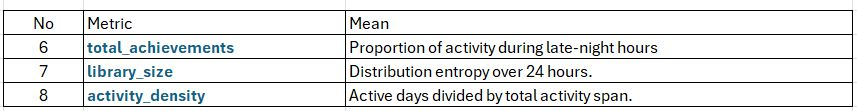
\includegraphics[width=0.7\linewidth]{Images/Slide/img167}
    }{
        \fbox{\begin{minipage}{0.7\linewidth}
            \centering
            \vspace{2cm}
            [IMAGE PLACEHOLDER]\\
            \texttt{Images/Slide/img167.jpg}\\
            \vspace{2cm}
        \end{minipage}}
    }
    \caption{Chi tiết các chỉ số hành vi của một tài khoản}
    \label{fig:dash_details}
\end{figure}


\begin{figure}[H]
    \centering
    \IfFileExists{Images/Slide/img172.jpg}{
        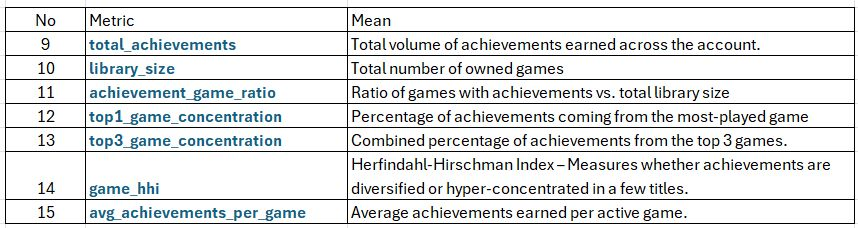
\includegraphics[width=0.7\linewidth]{Images/Slide/img172}
    }{
        \fbox{\begin{minipage}{0.7\linewidth}
            \centering
            \vspace{2cm}
            [IMAGE PLACEHOLDER]\\
            \texttt{Images/Slide/img172.jpg}\\
            \vspace{2cm}
        \end{minipage}}
    }
    \caption{So sánh 12 đặc trưng sai lệch nhất so với Baseline}
    \label{fig:comp_baseline}
\end{figure}


\subsection{Phân Tích Tổng Quan Dữ Liệu}

\begin{figure}[H]
    \centering
    \IfFileExists{Images/Slide/img177.jpg}{
        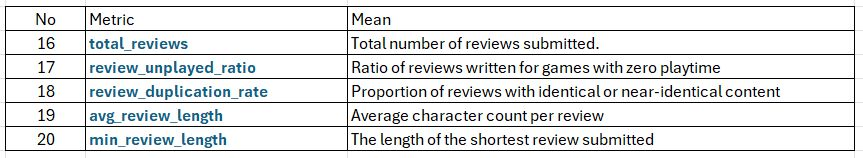
\includegraphics[width=0.7\linewidth]{Images/Slide/img177}
    }{
        \fbox{\begin{minipage}{0.7\linewidth}
            \centering
            \vspace{2cm}
            [IMAGE PLACEHOLDER]\\
            \texttt{Images/Slide/img177.jpg}\\
            \vspace{2cm}
        \end{minipage}}
    }
    \caption{Phân phối điểm Composite Score trong toàn bộ tập dữ liệu}
    \label{fig:dist_score}
\end{figure}


\begin{figure}[H]
    \centering
    \IfFileExists{Images/Slide/img182.jpg}{
        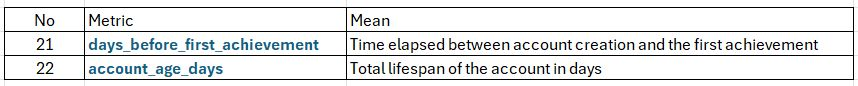
\includegraphics[width=0.7\linewidth]{Images/Slide/img182}
    }{
        \fbox{\begin{minipage}{0.7\linewidth}
            \centering
            \vspace{2cm}
            [IMAGE PLACEHOLDER]\\
            \texttt{Images/Slide/img182.jpg}\\
            \vspace{2cm}
        \end{minipage}}
    }
    \caption{Phân bố địa lý của các tài khoản bất thường}
    \label{fig:geo_dist}
\end{figure}

\begin{figure}[H]
    \centering
    \IfFileExists{Images/Slide/img183.jpg}{
        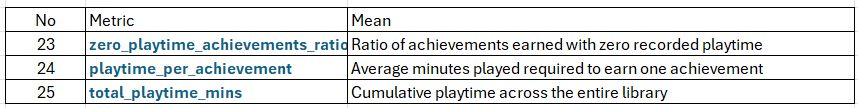
\includegraphics[width=0.7\linewidth]{Images/Slide/img183}
    }{
        \fbox{\begin{minipage}{0.7\linewidth}
            \centering
            \vspace{2cm}
            [IMAGE PLACEHOLDER]\\
            \texttt{Images/Slide/img183.jpg}\\
            \vspace{2cm}
        \end{minipage}}
    }
    \caption{Tương quan mô hình và Dashboard đồng thuận Ensemble}
    \label{fig:dash_consensus}
\end{figure}


\begin{figure}[H]
    \centering
    \IfFileExists{Images/Slide/img197.jpg}{
        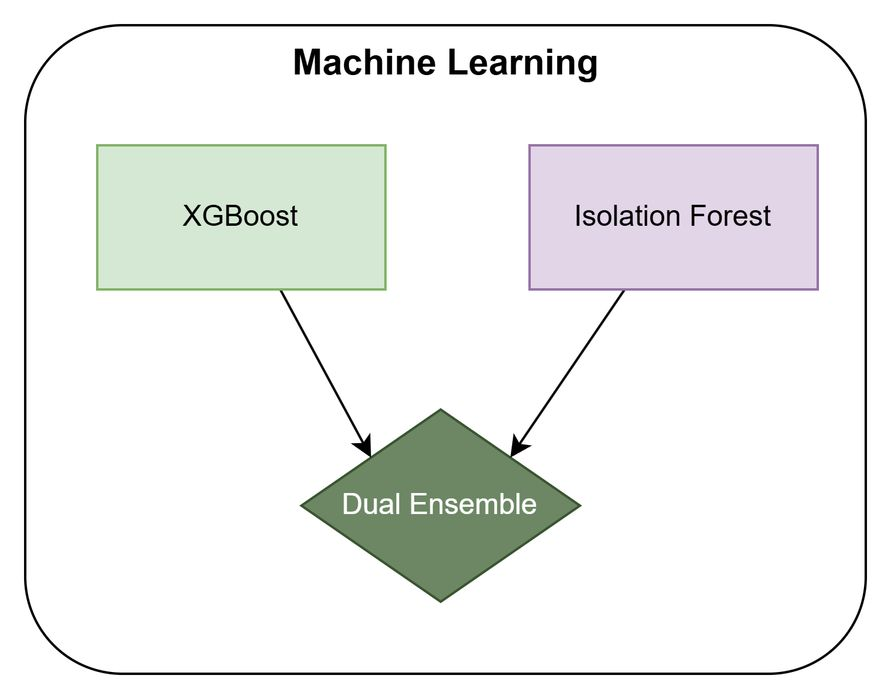
\includegraphics[width=0.7\linewidth]{Images/Slide/img197}
    }{
        \fbox{\begin{minipage}{0.7\linewidth}
            \centering
            \vspace{2cm}
            [IMAGE PLACEHOLDER]\\
            \texttt{Images/Slide/img197.jpg}\\
            \vspace{2cm}
        \end{minipage}}
    }
    \caption{Ma trận đồng thuận giữa XGBoost và Isolation Forest}
    \label{fig:consensus}
\end{figure}


\subsection{Phân Tích Đặc Trưng Discriminative}

\begin{figure}[H]
    \centering
    \IfFileExists{Images/Slide/img206.jpg}{
        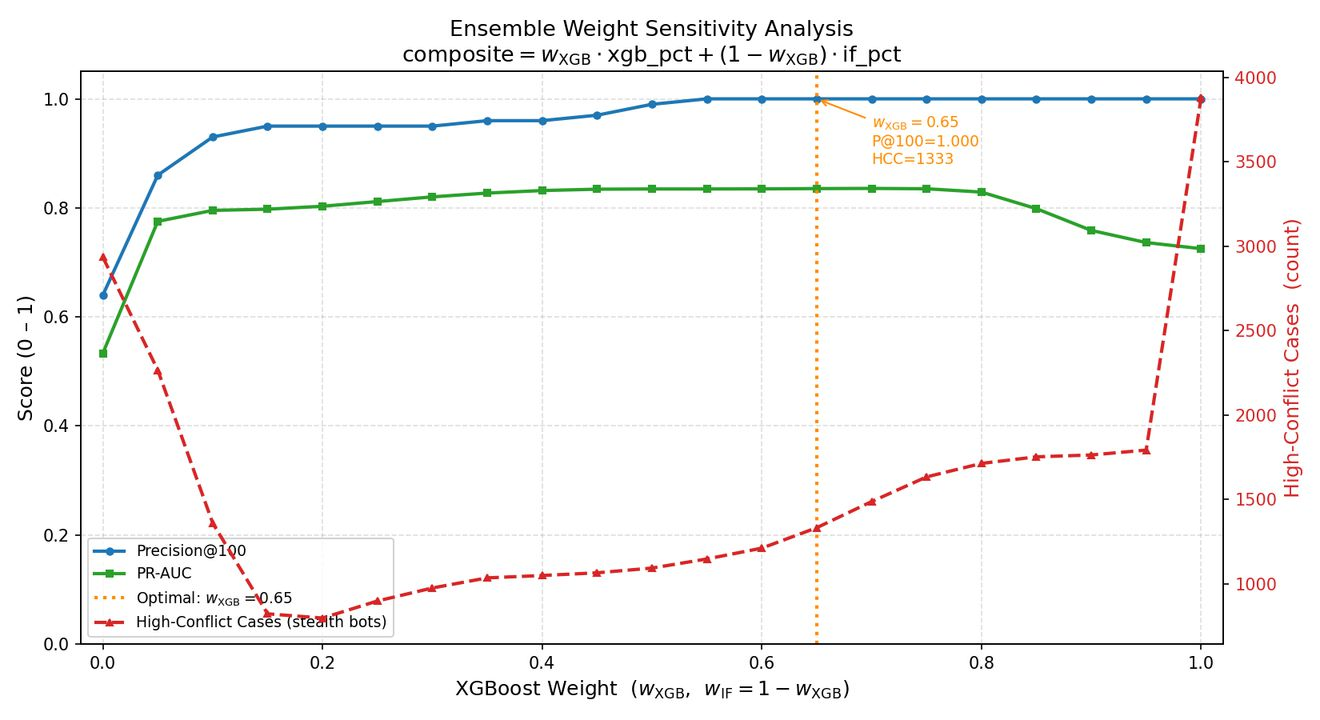
\includegraphics[width=0.7\linewidth]{Images/Slide/img206}
    }{
        \fbox{\begin{minipage}{0.7\linewidth}
            \centering
            \vspace{2cm}
            [IMAGE PLACEHOLDER]\\
            \texttt{Images/Slide/img206.jpg}\\
            \vspace{2cm}
        \end{minipage}}
    }
    \caption{So sánh tỷ lệ và chỉ số Cohen's d giữa nhóm Bot và Normal}
    \label{fig:effect_size}
\end{figure}


\begin{figure}[H]
    \centering
    \IfFileExists{Images/Slide/img211.jpg}{
        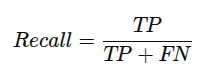
\includegraphics[width=0.7\linewidth]{Images/Slide/img211}
    }{
        \fbox{\begin{minipage}{0.7\linewidth}
            \centering
            \vspace{2cm}
            [IMAGE PLACEHOLDER]\\
            \texttt{Images/Slide/img211.jpg}\\
            \vspace{2cm}
        \end{minipage}}
    }
    \caption{Tương quan giữa độ tuổi tài khoản và hoạt động đánh giá}
    \label{fig:corr_behavior}
\end{figure}


\begin{figure}[H]
    \centering
    \IfFileExists{Images/Slide/img212.jpg}{
        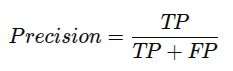
\includegraphics[width=0.45\linewidth]{Images/Slide/img212}
        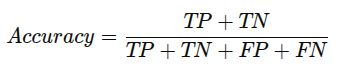
\includegraphics[width=0.45\linewidth]{Images/Slide/img213} \\
        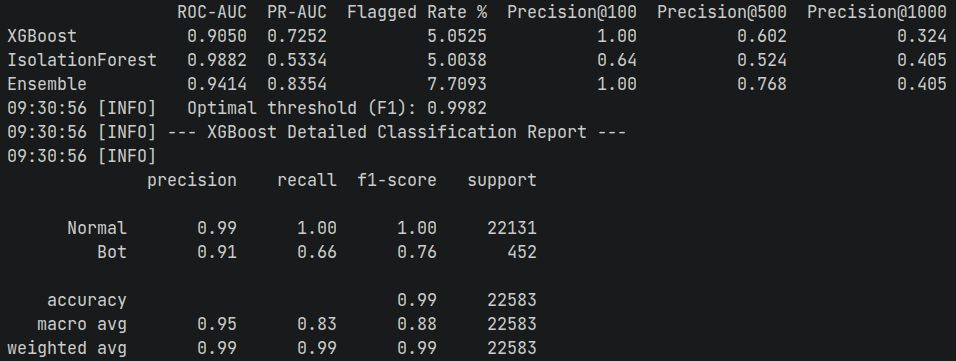
\includegraphics[width=0.45\linewidth]{Images/Slide/img218}
        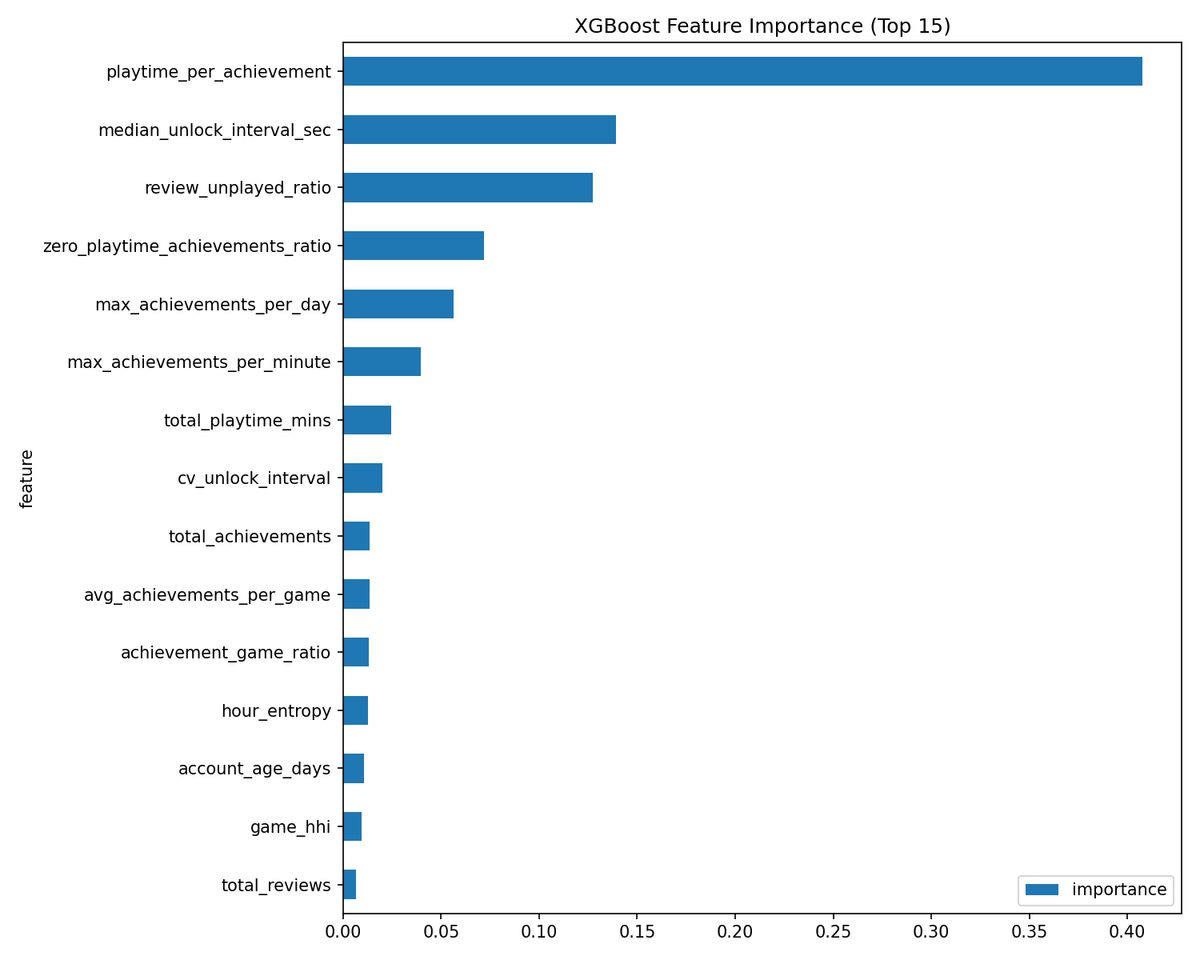
\includegraphics[width=0.45\linewidth]{Images/Slide/img223}
    }{
        \fbox{\begin{minipage}{0.7\linewidth}
            \centering
            \vspace{2cm}
            [IMAGE PLACEHOLDER]\\
            \texttt{Images/Slide/img212.jpg - img309.jpg}\\
            \vspace{2cm}
        \end{minipage}}
    }
    \caption{Tỷ lệ bất thường theo quy mô thư viện, thời gian chơi và năm tạo tài khoản}
    \label{fig:anomaly_rates}
\end{figure}



\section{Cải Tiến Liên Tục}

\subsection{Chu Kỳ}
\begin{enumerate}
    \item \textbf{Inference}: Dự báo trên dữ liệu mới
    \item \textbf{Active Learning}: Tạo mẫu conflict cho human review
    \item \textbf{Human Labeling}: Reviewer gán nhãn
    \item \textbf{Re-training}: Integrate human labels → train mô hình lại
    \item \textbf{Evaluation}: Đánh giá chất lượng → quay lại bước 1
\end{enumerate}

\subsection{Metrics Theo Dõi}
\begin{itemize}
    \item \textbf{ROC-AUC}: Không còn auto-flip; log để theo dõi chất lượng
    \item \textbf{PR-AUC}: Metric chính cho imbalanced data
    \item \textbf{Precision@Top-K}: Độ chính xác trong top-K suspicious accounts (K = 100, 500, 1000)
    \item \textbf{Human Agreement Rate}: Tỷ lệ mô hình dự báo đúng với human labels
\end{itemize}

\section{Tóm Tắt}
Giai đoạn dự báo \& ứng dụng bao gồm: (1) Inference trên dữ liệu mới, (2) Active Learning để xác định mẫu cần review, (3) Human-in-the-Loop labeling để cải thiện, (4) Đánh giá toàn diện chất lượng mô hình qua 4 nhóm metrics, (5) Chu kỳ cải tiến liên tục. Hệ thống được thiết kế để tăng độ chính xác \& độ tin cậy theo thời gian thông qua feedback từ human reviewers.
``

\section{Tóm Tắt}
Hệ thống không chỉ dừng lại ở dự báo tĩnh, mà còn đưa ra cấu trúc học tập vòng lặp (Active Learning) nhờ human-in-the-loop, bảo đảm mô hình ngày càng chính xác theo thời gian.

\newpage
\chapter{Đánh giá}

% TODO: Gom cụm, Chất lượng
\newpage

%%%%%%%%%%%%%%%%%OUTRO%%%%%%%%%%%%%%%%%%%
\newpage
\section{Phụ lục}
\subsection{ADR 01: Lựa chọn khung làm việc mạng giữa Unity Netcode và Photon Fusion 2} \label{adr:01}

\begin{enumerate}
	\item \textbf{Tiêu đề:} lựa chọn khung làm việc cho trò chơi nhiều người.
	\item \textbf{Trạng thái:} Đã chấp nhận.
	\item \textbf{Bối cảnh:}
	\begin{enumerate}
		\item Trò chơi yêu cầu kết nối tối đa 3 người chơi trong một trận đấu theo lượt, tốc độ chậm và không có giả lập vật lý phức tạp.
		\item Cần một hệ thống đóng gói tốt các chi tiết mạng cấp thấp để tập trung vào logic thẻ bài và tương tác với máy chủ phía sau.
		\item Đảm bảo tính ổn định của trạng thái trò chơi trên tất cả các máy khách mà không cần tự xây dựng lại các cơ chế bù lag hay dự đoán trạng thái.
	\end{enumerate}
	\item \textbf{Quyết định:}
	\begin{enumerate}
		\item Áp dụng \textbf{Photon Fusion 2} thay vì Netcode for GameObjects để tận dụng hệ thống quản lý trạng thái dựa trên tích tắc mạnh mẽ.
		\item Sử dụng chế độ \textbf{Shared Mode} để đơn giản hóa việc kết nối cho nhóm nhỏ và giảm chi phí vận hành máy chủ.
	\end{enumerate}
	\item \textbf{Hệ quả:}
	\begin{enumerate}
		\item \textbf{Tăng độ chính xác dữ liệu:} Nhờ vào cơ chế đồng bộ thuộc tính mạng thay vì gửi lệnh thủ công qua RPC.
		\item \textbf{Đường cong học tập cao hơn:} Đội ngũ phát triển cần làm quen với mô hình lập trình dựa trên tick thay vì hàm cập nhật truyền thống.
		\item \textbf{Đóng gói tốt hơn:} Tách biệt rõ ràng giữa dữ liệu mạng và logic hiển thị theo nguyên tắc \textbf{SOLID}.
	\end{enumerate}
\end{enumerate}

\subsection{ADR 02: Chuyển đổi hệ thống giao diện từ Legacy UI sang UI Toolkit} \label{adr:02}

\begin{enumerate}
	\item \textbf{Tiêu đề:} chuyển đổi từ hệ thống giao diện cũ sang ui toolkit.
	\item \textbf{Trạng thái:} Đã chấp nhận.
	\item \textbf{Bối cảnh:}
	\begin{enumerate}
		\item Mục tiêu áp dụng kiến trúc \textbf{MVC} để quản lý các lần gọi giao diện lập trình ứng dụng và cập nhật mô hình dữ liệu một cách nghiêm ngặt.
		\item Hệ thống giao diện cũ gây khó khăn trong việc tách biệt logic và thẩm mỹ, đồng thời thường xuyên gây xung đột dữ liệu khi làm việc nhóm trên các tệp đúc sẵn.
		\item Cần một giải pháp hỗ trợ \textbf{Data Binding} mạnh mẽ để tự động hóa việc hiển thị dữ liệu từ mô hình mà không cần viết mã thủ công quá nhiều.
	\end{enumerate}
	\item \textbf{Quyết định:}
	\begin{enumerate}
		\item Chuyển đổi toàn bộ hệ thống giao diện sang \textbf{UI Toolkit} trên Unity 6.
		\item Thực hiện gắn kết sự kiện hoàn toàn qua mã nguồn thay vì sử dụng cửa sổ thuộc tính để đảm bảo tính đóng gói và dễ kiểm thử.
	\end{enumerate}
	\item \textbf{Hệ quả:}
	\begin{enumerate}
		\item \textbf{Tuân thủ nguyên tắc DRY:} Quản lý style tập trung qua các tệp style dùng chung, tránh lặp lại định dạng cho từng thành phần.
		\item \textbf{Tối ưu hóa luồng dữ liệu:} Việc tách biệt cấu trúc giao diện và logic điều khiển giúp việc tích hợp với máy chủ phía sau trở nên minh bạch và dễ bảo trì hơn.
		\item \textbf{Hiệu suất cải thiện:} Giảm bớt gánh nặng tính toán bố cục nhờ vào cơ chế dàn trang dựa trên Flexbox và ảo hóa danh sách.
	\end{enumerate}
\end{enumerate}
\newpage
\renewcommand{\refname}{} 
\section{Tài liệu tham khảo}
\vspace{-\baselineskip}
\vspace{-\baselineskip}

\bibliographystyle{plainurl}
\nocite{*}
\bibliography{Outro/reference}


\end{document}
	
	
